\section{Supplemental}
\vfill

\setcounter{figure}{0}
\renewcommand{\thefigure}{S\arabic{figure}}
\setcounter{table}{0}
\renewcommand{\thetable}{S\arabic{table}}

\newpage
\begin{figure}
\centering 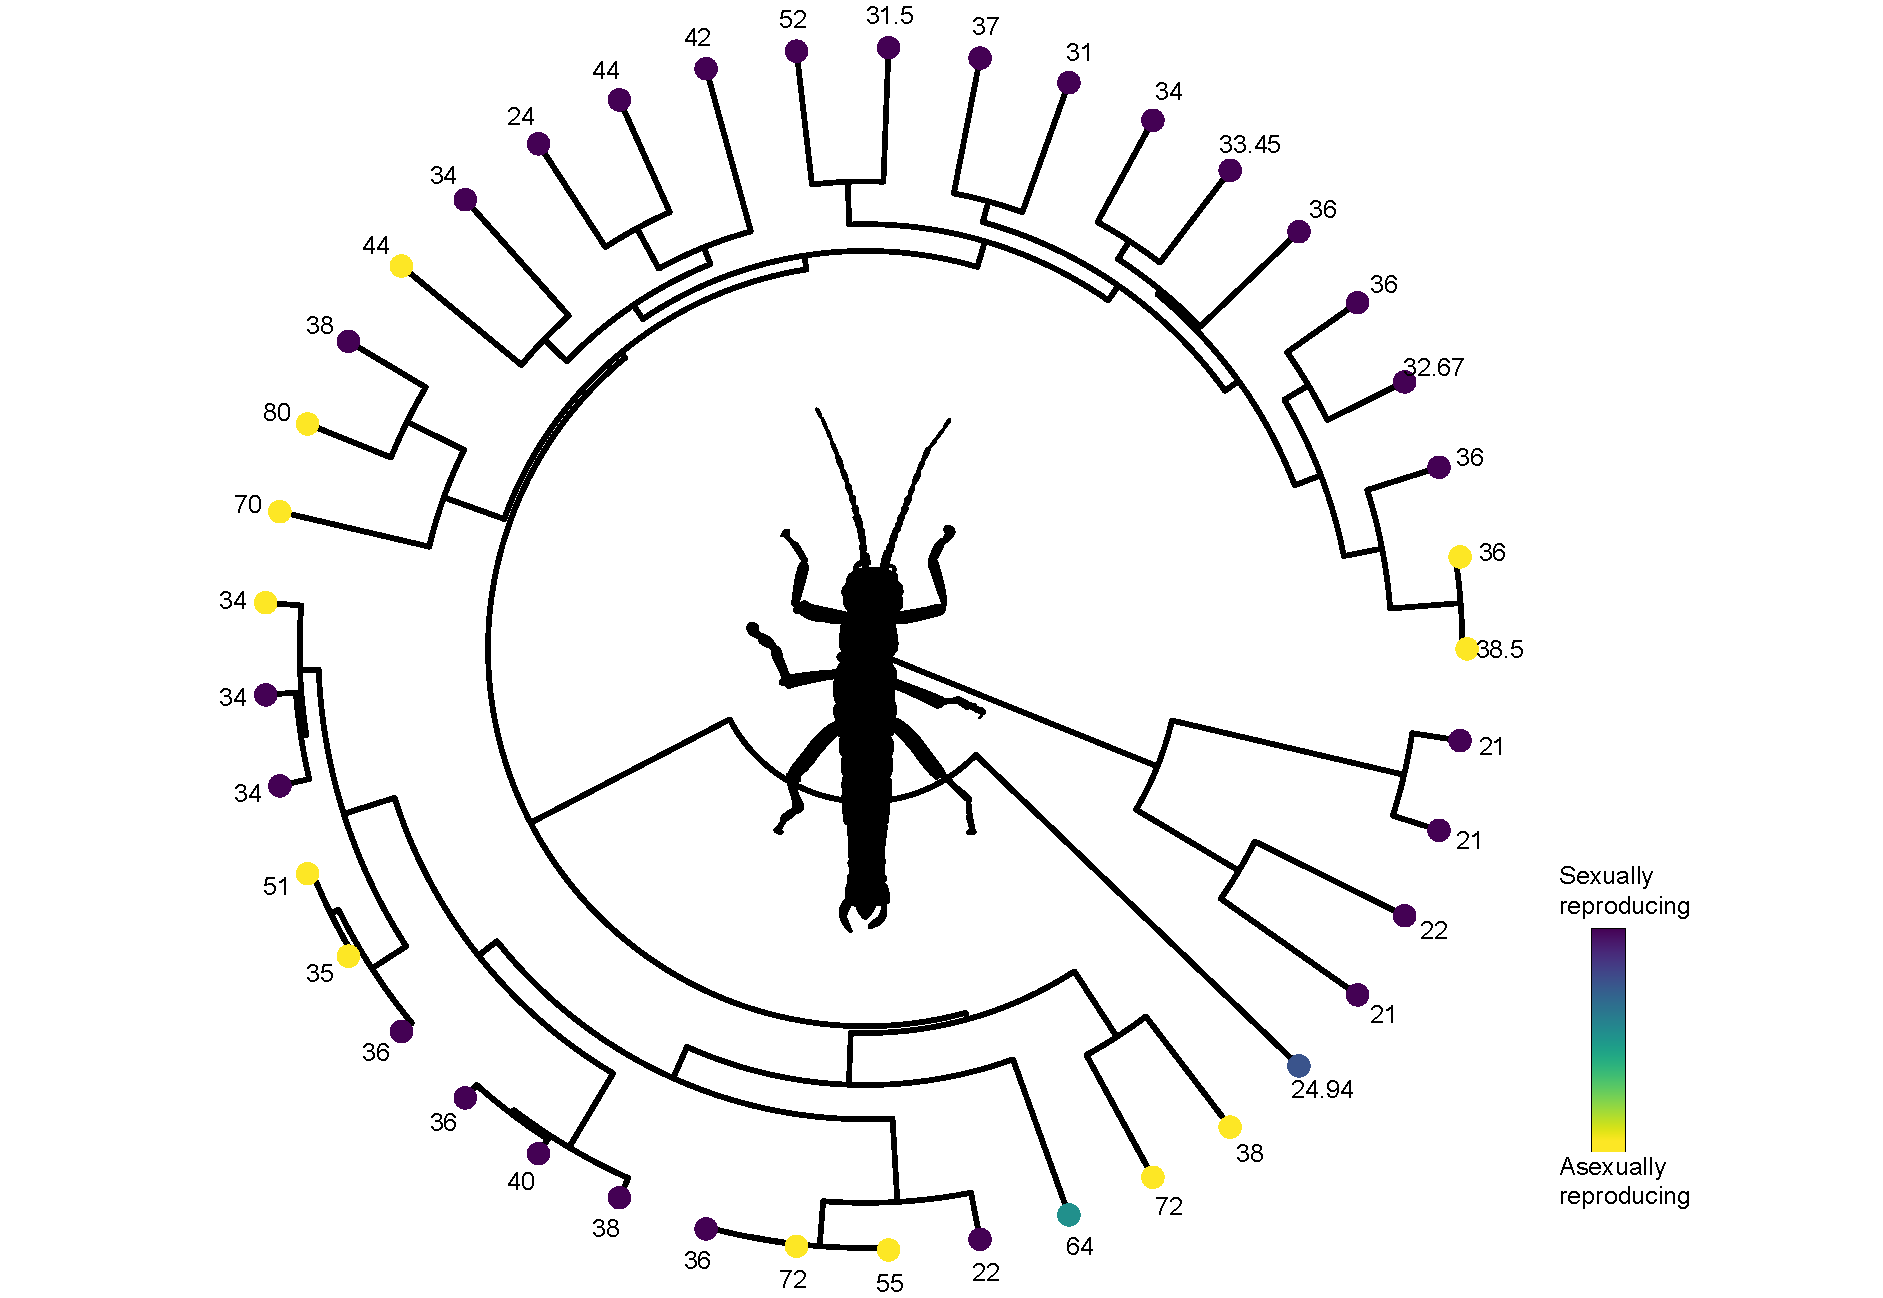
\includegraphics[width=1\textwidth]{figures/phasmatodea_phylogeny.pdf}
\caption{Phylogeny of the insect clade Phasmatodea. Tips are colored according to the mode of reproduction (sexual or asexual). Some lineages show intermediate colours. These are lineages which have both sexual and asexual populations. The shade of colour indicates the probability of observig either reproductive modes in these lineages. The numbers indicate the mean chromosome number for each lineage.}
\label{fig:phas.phylo}
\end{figure}

\begin{table}[ht]
\begin{tabular}{lcc}
\hline
\textbf{Transition} & \textbf{Mean rate (95\% credible interval)} & \textbf{Mean number of transitions} \\ \hline
XO to XY            & 0.0020 (0.0015 - 0.0026)                    & 15.3                                \\
XY to XO            & 0.0021 (0.0010 - 0.0036)                    & 6.7                                 \\ \hline
\end{tabular}
\caption{Mean transition rates and mean number of transitions obtained from stochastic mapping of sex chromosome transitions}
\label{tab:simmap.summary}
\end{table}
